\chapter{評価}
\label{chap:evaluation}

\section{評価手法}

\begin{figure}[htbp]
  \begin{center}
    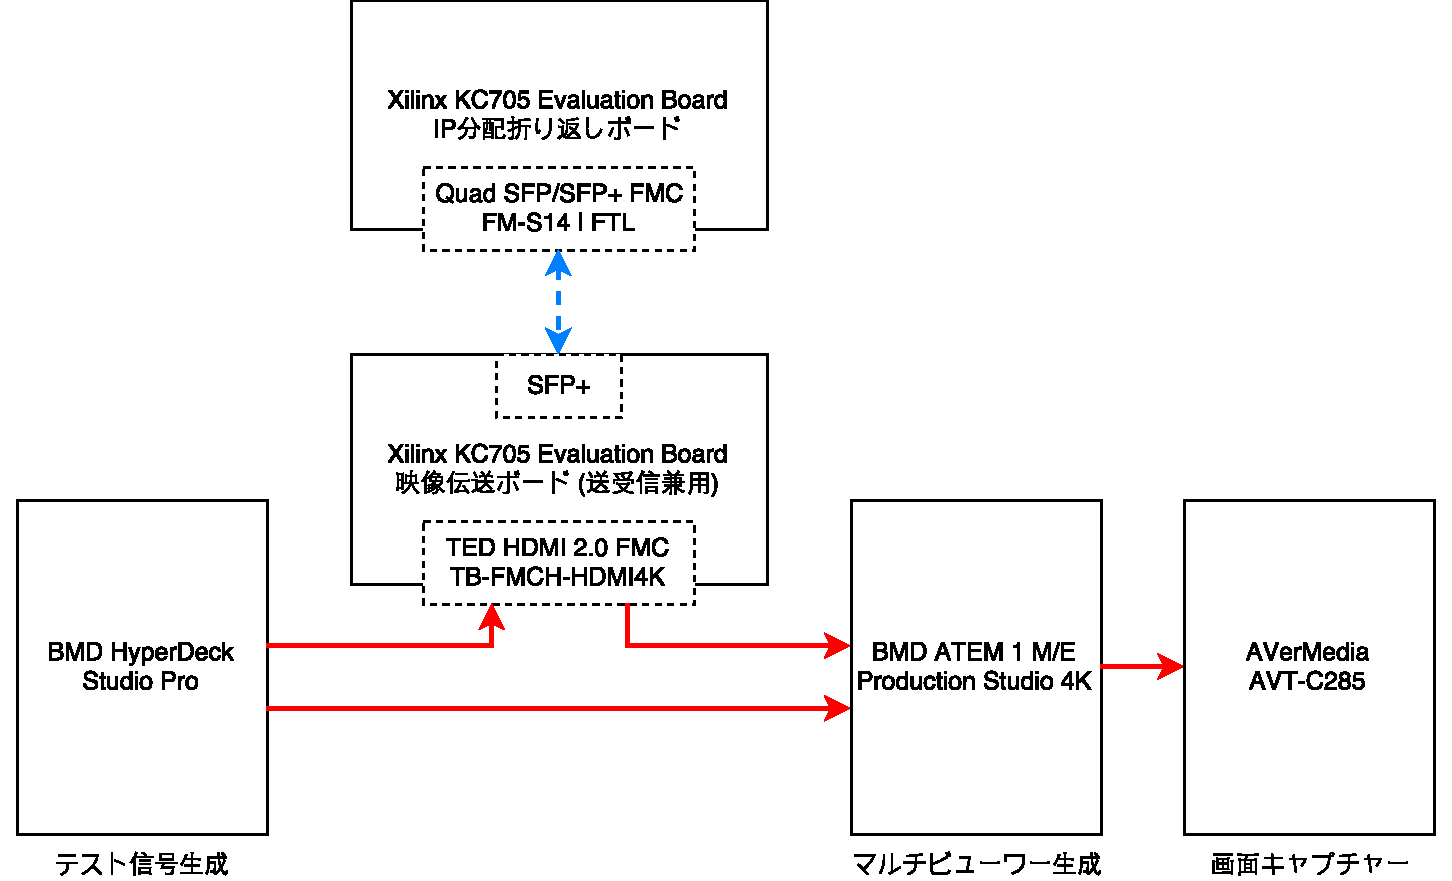
\includegraphics[bb=0 0 697 422,width=15.5cm]{img/evaluate-diagram.pdf}
  \end{center}
  \caption{ダイアグラム}
  \label{fig:evaluate-diagram}
\end{figure}

AAA

\section{計測}

BBB

図??のように計測を行った

\subsection{トラフィック}

CCC

\subsection{遅延}

DDD

\begin{table}[htbp]
  \caption{ソフトウェア実装による30FPSにおける遅延時間}
  \label{tb:pg235-vin-axi4-stream}
  \begin{center}
  \begin{tabular}{l|c|c}
    \hline
         & 遅延時間  & 遅延フレーム \\\hline\hline
    1回目 & 300 ms  & 9 frames \\\hline
    1回目 & 300 ms  & 9 frames \\\hline
    1回目 & 300 ms  & 9 frames \\\hline
    1回目 & 300 ms  & 9 frames \\\hline
    1回目 & 300 ms  & 9 frames \\\hline
    1回目 & 300 ms  & 9 frames \\\hline
    1回目 & 300 ms  & 9 frames \\\hline
    1回目 & 300 ms  & 9 frames \\\hline
    1回目 & 300 ms  & 9 frames \\\hline
    1回目 & 300 ms  & 9 frames \\\hline
    1回目 & 300 ms  & 9 frames \\\hline
    1回目 & 300 ms  & 9 frames \\\hline
    1回目 & 300 ms  & 9 frames \\\hline
    1回目 & 300 ms  & 9 frames \\\hline\hline
    平均  & 300 ms  & 9 frames \\\hline
  \end{tabular}\end{center}
\end{table}

\subsection{重量}

EEE

\subsection{安定性}

FFF

ケーブルを抜いた場合

徐々に遅延させていった場合

\section{実証実験}
本実装に実用性があることを顕彰するため、ORF2015とORF2016でそれぞれ実証実験を行った。
付録\ref{chap:orf2015}、付録\ref{chap:orf2016}

\section{考察}
